\documentclass[11pt]{article}
\usepackage{amsmath,amssymb}
\usepackage{booktabs}
\usepackage{threeparttable}
\usepackage{tabularx}
\usepackage{array}
\usepackage{graphicx}
\usepackage{microtype}
\usepackage{xcolor}
\usepackage{enumitem}
\usepackage{siunitx}
\usepackage{url}
\usepackage{hyperref}
\usepackage[capitalise,noabbrev]{cleveref}
\usepackage{lineno}
\usepackage{multirow}
\usepackage{longtable}
\usepackage{pdflscape}
\newcolumntype{L}{>{\raggedright\arraybackslash}X}
\newcolumntype{R}{>{\raggedleft\arraybackslash}X}
\newcommand{\code}[1]{\texttt{#1}}
\newcommand{\forum}{LabAutomation.io}
\newcommand{\repositoryurl}{https://github.com/fraware/lab-automation-observatory}
\newcommand{\pilotnote}{All quantitative results are bounded pilot estimates from purposively selected cases.}
\hypersetup{colorlinks=true,linkcolor=black,citecolor=blue!55!black,urlcolor=blue!60!black}
\setlist{nosep,leftmargin=*}
\sisetup{detect-all=true}
\Urlmuskip=0mu plus 2mu\relax
\emergencystretch=2em

\usepackage[margin=1in]{geometry}
\usepackage{authblk}

\title{The Lab Automation Observatory: A Reproducible Evidence Resource for Operational Knowledge in Digital Laboratories}
\author[1,2]{Mat\'eo H. Petel, M.S.}
\affil[1]{Center for Strategic Research in Critical Technologies}
\affil[2]{SentinelOps}
\date{}

\begin{document}
\maketitle

\begin{abstract}
Operational knowledge in laboratory automation is distributed across public discussions, vendor-specific explanations, local code, post-mortems, and transient support interactions. The Lab Automation Observatory converts a bounded public corpus into a versioned, machine-readable resource designed for audit, reuse, correction, and prospective study. The release contains 55 purposively selected discussion records, 45 analytical episodes, a ten-construct taxonomy, field-level metric inputs, source and claim audit ledgers, robustness analyses, JSON Schemas, executable analyses, regression tests, and governed example records. The resource preserves source provenance, unit, denominator, uncertainty, validation stage, known limitations, and prohibited inference. It also provides reusable schemas for reproducible troubleshooting questions, resolved-knowledge records, device-interface accessibility, and run events. We describe the resource architecture, construction, validation, empirical coverage, and intended reuse. The strongest pilot mechanism connects observability with recovery after irreversible physical execution, providing a prospective target for operational incident datasets. The Observatory is designed as infrastructure for studying and improving digital-laboratory practice; it is not an incident census, vendor benchmark, or verbatim forum archive.
\end{abstract}

\noindent\textbf{Keywords:} research resource; laboratory automation; data provenance; knowledge infrastructure; reproducibility; technical communities

\section{Context and motivation}

Laboratory automation depends on operational knowledge that is difficult to preserve as a conventional dataset. A device-integration answer can depend on model, firmware, licence, communication path, and software version. A method-reproduction question can depend on source files, external libraries, calibration, resource definitions, and active runtime state. A recovery decision can depend on which physical actions completed, where material remains, and which interventions occurred. Public technical communities record these details, although the information remains distributed across threads and its public outcome can be censored when work moves to private support or local implementation.

Existing integration standards and open frameworks improve machine interoperability \cite{bar2012sila,juchli2022sila2,porr2020gateway,bromig2022manager,wierenga2023pylabrobot}. Autonomous-laboratory research adds orchestration, adaptive experiment selection, and closed-loop execution \cite{abolhasani2023rise,hung2024community,canty2023autonomy,fei2024alabos,cousty2024glas}. These systems create demand for evidence objects that retain operational applicability, provenance, uncertainty, validation stage, maintenance ownership, and correction history.

The Lab Automation Observatory addresses this need through a derived and governed research resource. It converts a purposive public evidence base into typed records, bounded metrics, audit ledgers, reusable schemas, deterministic analyses, and versioned release artifacts. The resource is designed to support independent recoding, comparative schema work, prospective operational studies, and community knowledge stewardship. It excludes a verbatim forum archive and cannot support estimates of field prevalence, product reliability, installed base, or market share.

\section{Resource design principles}

The resource separates six objects that require different controls: source evidence, coded evidence, metric inputs, derived results, manuscript claims, and submission artifacts. A source record answers where the evidence came from and what context or wording was approved. A coded record states the analytical unit and construct assignment. A metric input preserves the eligible cases, component fields, unknown values, and denominator. A derived result is generated from those inputs. A claim record binds a manuscript statement to its evidence and prohibited overclaim. A release manifest binds the resulting files to immutable commits and hashes.

Four principles govern the representation.
\begin{enumerate}
  \item \textbf{Bounded units.} Every quantitative result names the object measured and its denominator.
  \item \textbf{Typed uncertainty.} Unknown, absent, partial, disputed, and superseded states remain distinct.
  \item \textbf{Validation-stage binding.} Logic, interface, simulation, dry, wet, assay, and production evidence support different claims.
  \item \textbf{Correctable provenance.} Records retain source links, applicability, date, ownership, limitations, and lineage.
\end{enumerate}

The design supports machine validation without implying that every field is objectively measurable or that ordinal rubric scores are probabilities. Human interpretation remains explicit in the codebook, episode notes, hard-case set, and claim ledger. Positive cases and counterexamples are retained so the resource represents successful infrastructure and correction processes alongside recurring gaps.

\section{Resource construction}

The pilot evidence base contains 55 purposively selected public discussions dated from 2022 through 2026. Selection sought conceptual coverage across platforms, workflow layers, incidents, design debates, documentation requests, product reports, vendor participation, and positive community outcomes. The thread served as the discovery unit. Fourteen deliberately difficult threads were segmented into 45 episodes so that interface access, deployment state, physical representation, observability, recovery, validation, and knowledge production could be represented separately when they occurred in one discussion.

The taxonomy contains ten constructs. B1 and B10 represent knowledge packaging and documentation or support. B2--B4 represent interface access, deployment identity, and physical resources. B5--B7 represent observability, recovery, and scheduling. B8 represents test--claim alignment. B9 represents AI context and physical feedback. Each code has inclusion, exclusion, primary-code, evidence, adjacency, and boundary rules.

All coding was performed by one analyst. The release reports no inter-rater statistic. A three-thread process-validation exercise identified ambiguities in the instrument and produced a primary-code tie-break, explicit read scopes, a formal episode unit, expected episode counts, and coherence tests. The answer-bearing key and a generated blind projection are released separately so that an independent coder can conduct a future pass without seeing the expected classifications.

Public-data handling follows a minimization strategy. The release contains derived records, short anonymized quotations, and source URLs. It excludes contributor handles, profile attributes, private messages, and a verbatim corpus. The source-audit ledger records approved quotation wording, context review, later-update checks, source role, and prohibited inference.

\section{Resource contents}

\subsection{Derived evidence records}

The thread register contains one row per selected discussion with title, date, category, source URL, primary code, direct-support codes, evidence type, public resolution, public artifact, migration status, evidence strength, and an analytical note. The episode register contains one row per segmented mechanism with lifecycle stage, primary technical code, ecosystem modifiers, evidence form, detectability, consequence, outcome, public artifact, counterexample status, and confidence. The hard-case table records likely disagreement, adjudication questions, required episode structure, and priority.

\subsection{Field-level metric inputs}

Separate files contain the cases underlying Integration Accessibility, Reproducibility Manifest Completeness, Physical Definition Completeness, Observability Coverage, Preflight Preventability, Constraint Completeness, Test--Claim Alignment, Context Expansion, and the documentation profile. Scores use 0, 0.5, and 1 where applicable, and unknown cells remain blank. Pairwise association files contain overlap, Jaccard similarity, lift, phi, conditional probabilities, descriptive risk ratios, and one-thread sensitivity.

\subsection{Robustness and audit records}

The robustness directory contains alternative partial-score weights, leave-one-thread-out association results, and defensible denominator alternatives. The source-audit ledger contains 25 independently addressable source records with canonical URLs and bibliography parity. The claim ledger records approved wording, evidence source, denominator, prohibited overclaim, limitation, and manuscript marker. Negative cases preserve public mechanisms that challenge an exclusively deficit-oriented account.

\subsection{Schemas and examples}

JSON Schemas define the minimum reproducible troubleshooting question, resolved-knowledge records, device-interface records, and run-event streams. Ten knowledge records demonstrate the governance model. Device-interface examples expose access components and limitations. Run-event examples illustrate linked commands, observations, interventions, recovery, and disposition for observability and partial-execution cases.

\subsection{Software and publication artifacts}

The Python package computes the released metrics, validates schemas, and exposes command-line reproduction. Scripts build derived files, robustness tables, figures, the graphical abstract, and submission bundles. Tests assert published values, identifier integrity, source mappings, generated-output synchronization, and fail-closed behavior. The LaTeX source, supplementary material, audits, manifests, and release hashes bind the analytical and publication layers.

\section{Validation and release controls}

Resource validation operates at several layers. Schema tests verify field types, required values, enumerations, identifiers, source domains, and conditional requirements. Cross-file tests verify that episodes reference existing threads, episode codes are supported at thread level, blind coding projections exclude answer-bearing fields, source-audit URLs match bibliography URLs, and approved quotations match the released quote bank.

Metric tests recompute every published value from the field-level inputs. Robustness tests regenerate alternative weighting, leave-one-thread-out, and denominator files and compare them with the committed outputs. Mutation tests alter selected inputs and require validation to fail, establishing that the release gates respond to material drift. Claim-traceability tests require each approved claim to appear at a marked manuscript location and retain an evidence source, denominator or qualitative scope, safe wording, prohibited overclaim, and limitation.

The certified v0.1.4 release passed 206 tests with 95.73\% branch-aware coverage. The release validator checked 31 CSV files, three robustness outputs, 25 source-audit rows, and 11 approved manuscript claims. The main manuscript, supplement, cover letter, and graphical abstract were rebuilt, checked for extractable text and embedded fonts, and inspected through rendered page images. A dual-SHA manifest distinguishes scientific source content from certification metadata and binds the canonical submission bundle to hashes.

These checks establish internal consistency, deterministic reproduction, and traceability. They do not establish representative sampling, independent coding agreement, or operational effectiveness of the proposed community artifacts. Those questions require the reuse studies described below.

\section{Intended use cases}

The resource supports five classes of use.

\begin{enumerate}
  \item \textbf{Independent qualitative replication.} A coder can analyze the blind hard-case set from the linked public sources and compare classifications only after submission.
  \item \textbf{Cross-community evidence studies.} Researchers can apply the unit, provenance, uncertainty, and claim-boundary pattern to another specialist technical community and compare which constructs transfer.
  \item \textbf{Laboratory knowledge stewardship.} Teams can adapt the question and resolved-knowledge schemas for internal or public support systems while retaining applicability, evidence, ownership, and expiry.
  \item \textbf{Operational instrumentation.} Laboratories can use the interface and event schemas to collect real integration and incident data with denominators unavailable in forum evidence.
  \item \textbf{AI-method evaluation.} Benchmark designers can construct missing-context tasks and report performance separately across syntactic, simulation, dry, wet, assay, and production stages.
\end{enumerate}

The resource should be evaluated by outcomes appropriate to each use. Coding replication requires agreement and adjudication records. Knowledge interventions require clarification burden, resolution time, recurrence, staleness, and correction latency. Interface registries require integration time, executable-device coverage, and failed dispatches. Event models require diagnosis time, safe-state time, salvage, final disposition, and recurrence. AI benchmarks require clarification quality, unsafe omission, human correction, and validation-stage performance.

The resource should not be used to infer vendor reliability, market position, installed base, contributor competence, or field-wide failure incidence. Those interpretations lack the required sampling frame and operational denominator.

\section{Empirical demonstration}

The resource was applied to nine bounded analytical objects. Mean Integration Accessibility was 63.9\% across six device--interface cases. Reproducibility Manifest Completeness was 54.2\% across three deployment objects. Physical Definition Completeness was 67.0\% across four resource cases, and Observability Coverage was 52.5\% across four execution or diagnostic cases. Two of three definitely classified partial-execution scenarios were preflight preventable, with an all-case sensitivity interval from 50.0\% to 75.0\%. A scheduling toy problem surfaced seven of eight incomplete requirement classes without resolving any to a scenario-specific value. Two of six bounded claims fully aligned test object, environment, acceptance rule, evidence, and claim scope. An AI-method discussion expanded from five opening context classes by ten core and seventeen broader reply-added classes. Five of twelve documentation-centered cases received a fully actionable public outcome.

The component metrics were recomputed with alternative partial-score weights from 0 through 1. Their central values depend on the conventional representation of partial evidence, confirming that they should be read as ordinal rubric summaries. Pairwise analysis among B2--B9 identified observability--recovery as the strongest relationship ($\phi=0.452$, lift $=2.353$). Leave-one-thread-out deletion retained the relationship above the pilot attention threshold in all 55 deletions. Observability--validation and interface accessibility--scheduling were also stable priorities. The validation--AI relationship remained exploratory because the AI stratum was small and threshold retention was limited.

These results demonstrate the resource's ability to preserve heterogeneous evidence, compute bounded summaries, expose sensitivity, and bind interpretations to source and denominator. They do not establish that the corpus represents the broader laboratory-automation field.

\begin{figure}[t]
  \centering
  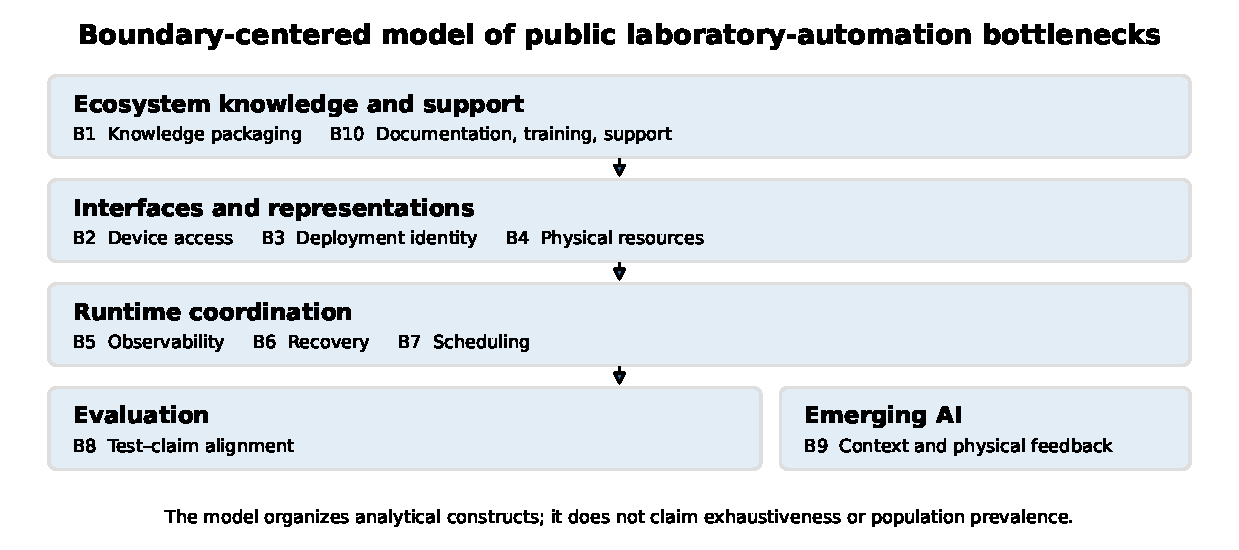
\includegraphics[width=\linewidth]{figures/conceptual_model.pdf}
  \caption{The released ten-construct model organizes ecosystem knowledge, interfaces and representations, runtime coordination, evaluation, and AI-specific context.}
\end{figure}

\begin{table}[t]
\centering
\caption{Bounded pilot metrics. Each row has a distinct unit and denominator.}
\label{tab:headline-metrics}
\begin{threeparttable}
\begin{tabularx}{\linewidth}{@{}L r l L@{}}
\toprule
Construct & Result & 95\% Wilson & Unit and denominator \\
\midrule
B2 Integration accessibility & 63.9\% & -- & 6 device--interface cases \\
B3 Deployment manifest & 54.2\% & -- & 3 deployment objects; 24 applicable cells \\
B4 Physical definitions & 67.0\% & -- & 4 resource definitions \\
B5 Observability & 52.5\% & -- & 4 execution/diagnostic cases \\
B6 Preflight preventability & 66.7\% & 20.8--93.9\% & 3 definite scenarios of 4 eligible \\
B7 Constraint discovery & 87.5\% & 52.9--97.8\% & 8 incomplete fields of 13 \\
B8 Fully aligned claims & 33.3\% & 9.7--70.0\% & 6 bounded claims \\
B9 Core context expansion & 2.0$\times$ & -- & 5 opening classes \\
B10 Actionable public outcome & 41.7\% & 19.3--68.0\% & 12 documentation cases \\
\bottomrule
\end{tabularx}
\begin{tablenotes}[flushleft]\footnotesize
\item Results demonstrate operationalization in selected cases. They do not estimate forum-wide or industry-wide rates.
\item Wilson intervals are descriptive uncertainty for the stated denominator, not population inference. A dash marks a row whose result is a mean of ordinal component scores or a ratio rather than a proportion, for which a binomial interval would be undefined.
\item Component means are taken over known cells only; unknown cells are excluded rather than scored as zero.
\end{tablenotes}
\end{threeparttable}
\end{table}


\section{Limitations and responsible use}

The evidence base is purposive, single-coder, and limited to one public specialist community. It was constructed to maximize conceptual coverage and metric design, not representativeness. Public discussion is shaped by installed base, product complexity, community participation, shareability, and migration to private support. Open thread status cannot be equated with operational non-resolution.

The field-level case sets are small and heterogeneous. Their scores demonstrate operationalization and expose missing fields; they are not calibrated probabilities or common performance measures. Pairwise associations arise from multi-label coding in a purposive corpus and remain descriptive. Source-reported product evidence has not been converted into independent replication. The community schemas are designed artifacts whose operational value remains to be evaluated.

Responsible reuse requires preservation of the original analytical unit, denominator, uncertainty state, validation stage, and prohibited inference. Users should retain source provenance and contributor ownership, avoid redistributing copied discussions, and document corrections through explicit versioning and lineage. Extension to another domain should include domain-specific code boundaries and independent validation instead of assuming that the ten constructs are exhaustive.

\section{Availability, maintenance, and outlook}

The certified v0.1.4 release is available at \url{https://github.com/fraware/lab-automation-observatory/releases/tag/v0.1.4}. A persistent archive DOI must be inserted before a Patterns submission. The repository provides machine-readable data, schemas, software, tests, documentation, LaTeX source, release audits, and hashes. Code is licensed under Apache-2.0. Original documentation and derived data are licensed under CC BY 4.0. Quoted forum text remains subject to the rights of its original authors.

The project uses explicit record status and supersession. Future source corrections, coding changes, or claim-affecting changes require a new version and updated derived outputs, tests, audit, and manifest. The roadmap prioritizes independent recoding, evaluation of the question and knowledge interventions, prospective observability--recovery data, expanded interface records, and cross-community application.

The Observatory demonstrates a general resource pattern for operational knowledge that spans public discourse, structured evidence, executable analysis, and community infrastructure. Its long-term value will depend on demonstrated reuse outside the initiating pilot. That requirement motivates the editorial inquiry and additional adoption evidence specified in the accompanying venue checklist.

\section*{Author contributions}
Mat\'eo H. Petel: Conceptualization, methodology, investigation, data curation, software, formal analysis, visualization, writing, and project administration.

\section*{Declaration of interests}
The author declares no competing financial or commercial interest.

\section*{Funding}
This work received no specific grant from any funding agency.

\section*{Use of generative AI}
OpenAI ChatGPT assisted with language editing, code scaffolding, consistency checks, and artifact formatting. The author reviewed all generated material and accepts responsibility for the resource and manuscript.


\bibliographystyle{unsrt}
\bibliography{references}
\end{document}
